% EN48 c06 | 原书 p.82–91 上部（PDF 91–100） | 第 4 章 §4.1
% 边界调整：原定 p.82–90；§4.1 末尾（本块最后一条断言的证明）跨到 p.91 上半，
% 为使小节与编号完整，本块补译 p.91 上半至 §4.2 标题之前（§4.2 起属下一块）。
\section{深谷范畴}

\subsection{$Y$ 的 Fukaya--Seidel 范畴：引言}

% ===== 原书 p.82 =====
辛流形上的深谷范畴、辛纤维丛上的 Fukaya--Seidel 范畴，都是 $A_\infty$-范畴。下文考虑
$v_0\colon Y\to\C$ 的 Fukaya--Seidel 范畴的一个子范畴。随后我们过渡到上同调层面
（在此 $A_\infty$-范畴成为普通范畴），证明该子范畴等价于超曲面 $H=\Sigma_2$ 上相干层的
有界导出范畴。

\transnote{「过渡到上同调层面」指把 $A_\infty$-范畴的态射空间取上同调：当 $\mu^1=0$
时，$\mu^2$ 诱导出普通范畴的复合。下文的一切等价都在这个层面上陈述，故不必显式处理
更高的 $A_\infty$ 积。}

\begin{remark}[非正合、非紧，且不用哈密顿扰动方法]\label{rem:4-1-1}
在 [Sei08] 中，Lefschetz 纤维丛的深谷范畴以顶针（Lefschetz thimble）为拉格朗日对象：
把球面平行移动到 Morse 奇异纤维中的奇点处，球面在此被掐成一点。我们的情形不同：
$0$ 上的退化纤维不是 Lefschetz 奇点（即不是局部模型 $\sum_i|z_i|^2$），而是 $T^4$
沿一族 $S^1$ 收缩、并在两个点处再收缩一个 $T^2$ 而退化。因此我们改为考虑绕该奇异
纤维一周的拉格朗日对象，并令其在无穷远处有由超势 $v_0$ 控制的行为。这是因为它乃是
两个平行移动到中心纤维的纤维拉格朗日的磨光（smoothing）。这就是 [AS] 中 U 形曲线
（U-shaped curve）的概念。
\end{remark}

\transnote{顶针沿 Lefschetz 纤维丛的消失道路把球面收缩到奇点；本文的退化纤维不是
Lefschetz 奇点，而是 $T^4$ 的「薄化」，故拉格朗日对象要绕着奇异纤维走。U 形曲线可
设想为两条平行移动到中心纤维的纤维拉格朗日被磨光后连成的一条曲线。}

我们的设定与 [Sei08] 的第一点差别是：这里是非正合情形，因此会出现球泡
（sphere bubble）。另外，纤维丛 $v_0$ 的底空间所在的流形非紧；等价地，我们可以限制到
原点的一个邻域，此时流形带边界。第二点差别是：Seidel 在后来的若干论文中虽在 U 形
曲线上定义深谷范畴，但他使用的哈密顿扰动要求辛形式在底与纤维上是乘积形式。这里的
辛形式不是乘积形式，所以我们改用 [AS] 与 Ganatra 讲义中的范畴局部化
（categorical localization）概念。

\begin{example}[非单调]\label{ex:4-1-2}
我们也不处在单调（monotone）设定中，而这是另一套标准设定。为了说明单调性，我们
借用 Oh 关于 Clifford 环面的如下例子 [Oh93]。
\end{example}

% ===== 原书 p.83 =====
\begin{definition}[映射的 Maslov 指数]\label{def:4-1-3}
给定 $u\colon(\mathbb{D},\partial\mathbb{D})\to(M,L)$，先把 $u^*TM$ 在盘上平凡化。
于是 Maslov 指数（Maslov index）计算 $\R$ 在该平凡化拉回中绕边界的旋转圈数。
\end{definition}

\begin{definition}\label{def:4-1-4}
辛流形 $(M,\omega)$ 中的拉格朗日子流形 $L$ 称为\textbf{单调的}（monotone），若存在
常数 $k$ 使得对一切 $u\in\pi_2(M,L)$ 都有 $[\omega]=k\cdot[\mu(u)]$。也就是说，
盘的面积与这些盘的 Maslov 指数成比例。
\end{definition}

\transnote{单调性要求比例常数 $k$ 与盘 $u$ 无关；这是排除球泡、保证 Floer 理论良
定义的标准设定之一。本文既非正合也非单调，故须另行处理球泡。}

在 $L\iso T^n$ 为 Clifford 环面、$M:=\PP^n$ 的情形，为得到 $\pi_2(M,L)$，可用空间偶
的同伦正合列得到分裂正合列（之所以分裂，是因为边界同态有由包含诱导的逆映射）；
随后 $\pi_2(\PP^n)$ 由纤维丛 $S^1\to S^{2n+1}\to\PP^n$ 的同伦正合列给出。

由此得到 $H_2(M,L)$ 的一组基，在这组基上检验 Maslov 指数与面积成比例即可。事实上
只需检查两个元素，因为 Clifford 环面 $T^n$ 中其余元素由对称性给出同样的结果。在
$T^n$ 中，映射 $w_k(z)=[1:\cdots:0:z:0\cdots:0]$（$k>0$）的指数为 $2$，因为我们
转了一整圈，于是直线 $\R$ 被旋转了两次。

两条映射 $u$ 与 $u'$（满足 $u|_{\partial\mathbb{D}}=u'|_{\partial\mathbb{D}}$）的
Maslov 指数之差为 $\int_{u(\mathbb{D}^2)\cup u'(\mathbb{D}^2)}2c_1(M)$。于是由
$\{[z:0:\cdots:0]\}_{z\in\mathbb{D}}$ 定义的盘映射 $w_0\colon\mathbb{D}\to M$ 的
Maslov 指数为 $2c_1(\PP^n)=2(n+1)$；这是因为可把 $w_0$ 看作粘上一个常值盘，或等价地
看作把球面经由细管粘到 $T^n$ 上，所用的正是 $\pi_2(\PP^n)$ 的生成元在同伦长正合列
下的像。最终得到
\[
\frac{\operatorname{Area}(w_1)}{\operatorname{Area}(w_0)}
=\frac{1}{n+1}=\frac{\mu(w_1)}{\mu(w_0)}.
\]
本文所考虑的盘一律 Maslov 指数为 $2$，但面积按 [CO06] 的公式变化，这一点后文再详细
说明。

至此我们说明了本设定与现有文献中诸设定的差别，下面概述各节安排：先定义
Fukaya--Seidel 范畴，再证明 HMS 陈述。在 §4、§4、§4 三节中我们讨论绕
$v_0\colon Y\to\C$ 中心纤维的单值性，因为定义我们所考虑的 $FS(Y,v_0)$ 子范畴中的
拉格朗日对象需要它。随后 §4.2 建立定义 $H^0FS(Y,v_0)$ 中结构映射所需的背景，
§4.3 证明这些结构映射涉及的模空间满足可写入定义的条件。最后在 §4.4 给出定义，
并证明它在正则选取数据时良定义。

% [Tutor Note: 原书此处印作「In Sections 4, 4, and 4」，三个交叉引用编号在排版中
% 丢失（疑为 \ref 展开失败），保留原样并加译注。]

\medskip\noindent\textbf{单值性背景}\par
我们先定义单值性。我们正是靠它把纤维中的拉格朗日对象平行移动，从而得到全空间中的
拉格朗日对象。我们将在局部卡中定义 Darboux 坐标（也叫作用--角坐标），以便在深谷
范畴中做辛几何计算。

% ===== 原书 p.84 =====
\begin{definition}\label{def:4-1-5}
\textbf{辛纤维丛}（symplectic fibration）是指带有纤维丛结构的辛流形 $(Y,\omega)$，
且该纤维丛的纤维关于 $\omega$ 是辛的。
\end{definition}

\begin{example}\label{ex:4-1-6}
本文构造 $(Y,\omega)$ 时已使 $v_0\colon Y\to\C$ 成为辛纤维丛。
\end{example}

\begin{definition}\label{def:4-1-7}
辛纤维丛 $\pi\colon Y\to C$（底流形为 $C$）的\textbf{辛水平分布}
（symplectic horizontal distribution）是子丛 $H\subset TY$：若 $F$ 是 $\pi$ 的一般
纤维，则 $H=TF^{\omega}$ 为其 $\omega$-正交补，即
\[
\omega(H,TF)=0.
\]
\end{definition}

\begin{definition}\label{def:4-1-8}
给定两点 $p_0,p_1\in C$ 与连接它们的道路 $\gamma\colon I\to C$（即 $\gamma(0)=p_0$、
$\gamma(1)=p_1$），\textbf{平行移动映射}（parallel transport map）是辛同胚
$\Phi\colon F_{p_0}\to F_{p_1}$，定义如下：对 $x\in F_{p_0}$ 与 $v\in T_xF_{p_0}$，
令 $\Phi(x)$ 为 $\tilde\gamma(1)$，其中 $\tilde\gamma\colon I\to Y$ 满足
$\pi\circ\tilde\gamma=\gamma$、$d\pi(\tilde\gamma')=\gamma'$，且 $\tilde\gamma'$ 落在
水平分布中。
\end{definition}

\begin{remark}\label{rem:4-1-9}
上述最后一个条件保证 $\Phi$ 是辛同胚。
\end{remark}

\begin{definition}\label{def:4-1-10}
\textbf{单值性}（monodromy）是绕底空间中一个奇点一周的平行移动。
\end{definition}

本节的主要结果如下，见图~\ref{fig:4-1}：

\begin{lemma}\label{lem:4-1-11}
平行四边形 $T_B$ 的每个格中的单值性如下：远离热带曲线时，在上右角得到 $(0,0)$，
此处 $r_z^{-1}\gg r_x^{-1},r_y^{-1}$；在右侧得到 $(0,1)$，此处 $r_y^{-1}$ 最大；
在左侧得到 $(1,0)$，此处 $r_x^{-1}$ 最大；于是左下角得到 $(1,1)$。
\end{lemma}

\transnote{「远离热带曲线」指 $|x|,|y|,|z|$ 三者相对大小的三个区域，$r_x,r_y,r_z$
分别度量这三者。图~\ref{fig:4-1} 的四个格标出的正是单值性在 $H_1$ 中的像。}

\begin{remark}\label{rem:4-1-12}
我们对图~\ref{fig:4-1} 所画的几何作几句说明。$v_0$-纤维 $\Vdual$ 可用作用--角坐标
$(\xi_1,\xi_2,\theta_1,\theta_2)$ 描述。线性拉格朗日对象 $\ell_i$ 是 $\xi:=(\xi_1,\xi_2)$
上线性函数的图像；换言之，它以六边形为参数域。当我们把 $\Vdual$ 绕原点平行移动时，
$\phi(\ell_i)$ 仍以六边形为参数域，但角度按单值性发生了旋转。这一点下面会算。
\end{remark}

\begin{claim}\label{clm:4-1-13}
$\phi(\ell_i)$ 是 $(\Vdual,\restr{\omega}{\Vdual})$ 中的拉格朗日对象；由于 $v_0$ 关于
$\omega$ 是辛纤维丛，$\restr{\omega}{\Vdual}$ 也是辛形式。
\end{claim}

\begin{proof}
平行移动由取 $H:=(TF)^{\omega}$（纤维的辛正交补）定义。故单值性是辛同胚（参见
[MS17]），从而保持拉格朗日对象。
\end{proof}

\transnote{关键在水平分布的定义：$H$ 取纤维的辛正交补，故沿底空间道路的平行移动
保持 $\omega$；单值性作为绕奇点一周的平行移动，自然是辛同胚。}

\begin{remark}[记号]\label{rem:4-1-14}
令 $F:=\Vdual$；此后 $F$ 将指定义辛形式的凯勒势（Kähler potential）函数，而 $v_0$
的纤维记作 $\Vdual$。
\end{remark}

% [Tutor Note: 原书此注自相矛盾：先令 F:=V∨，随即又称 F 指凯勒势、纤维记作 V∨。
% 后文 p.86 中 F 确为凯勒势（ι_{Xi}((i/2π)∂∂̄F)），而最后一条断言的证明中 F 又指
% 纤维。保留原样并加译注，请读者按上下文判断。]

% ===== 原书 p.85 =====
\begin{figure}[htbp]
\centering
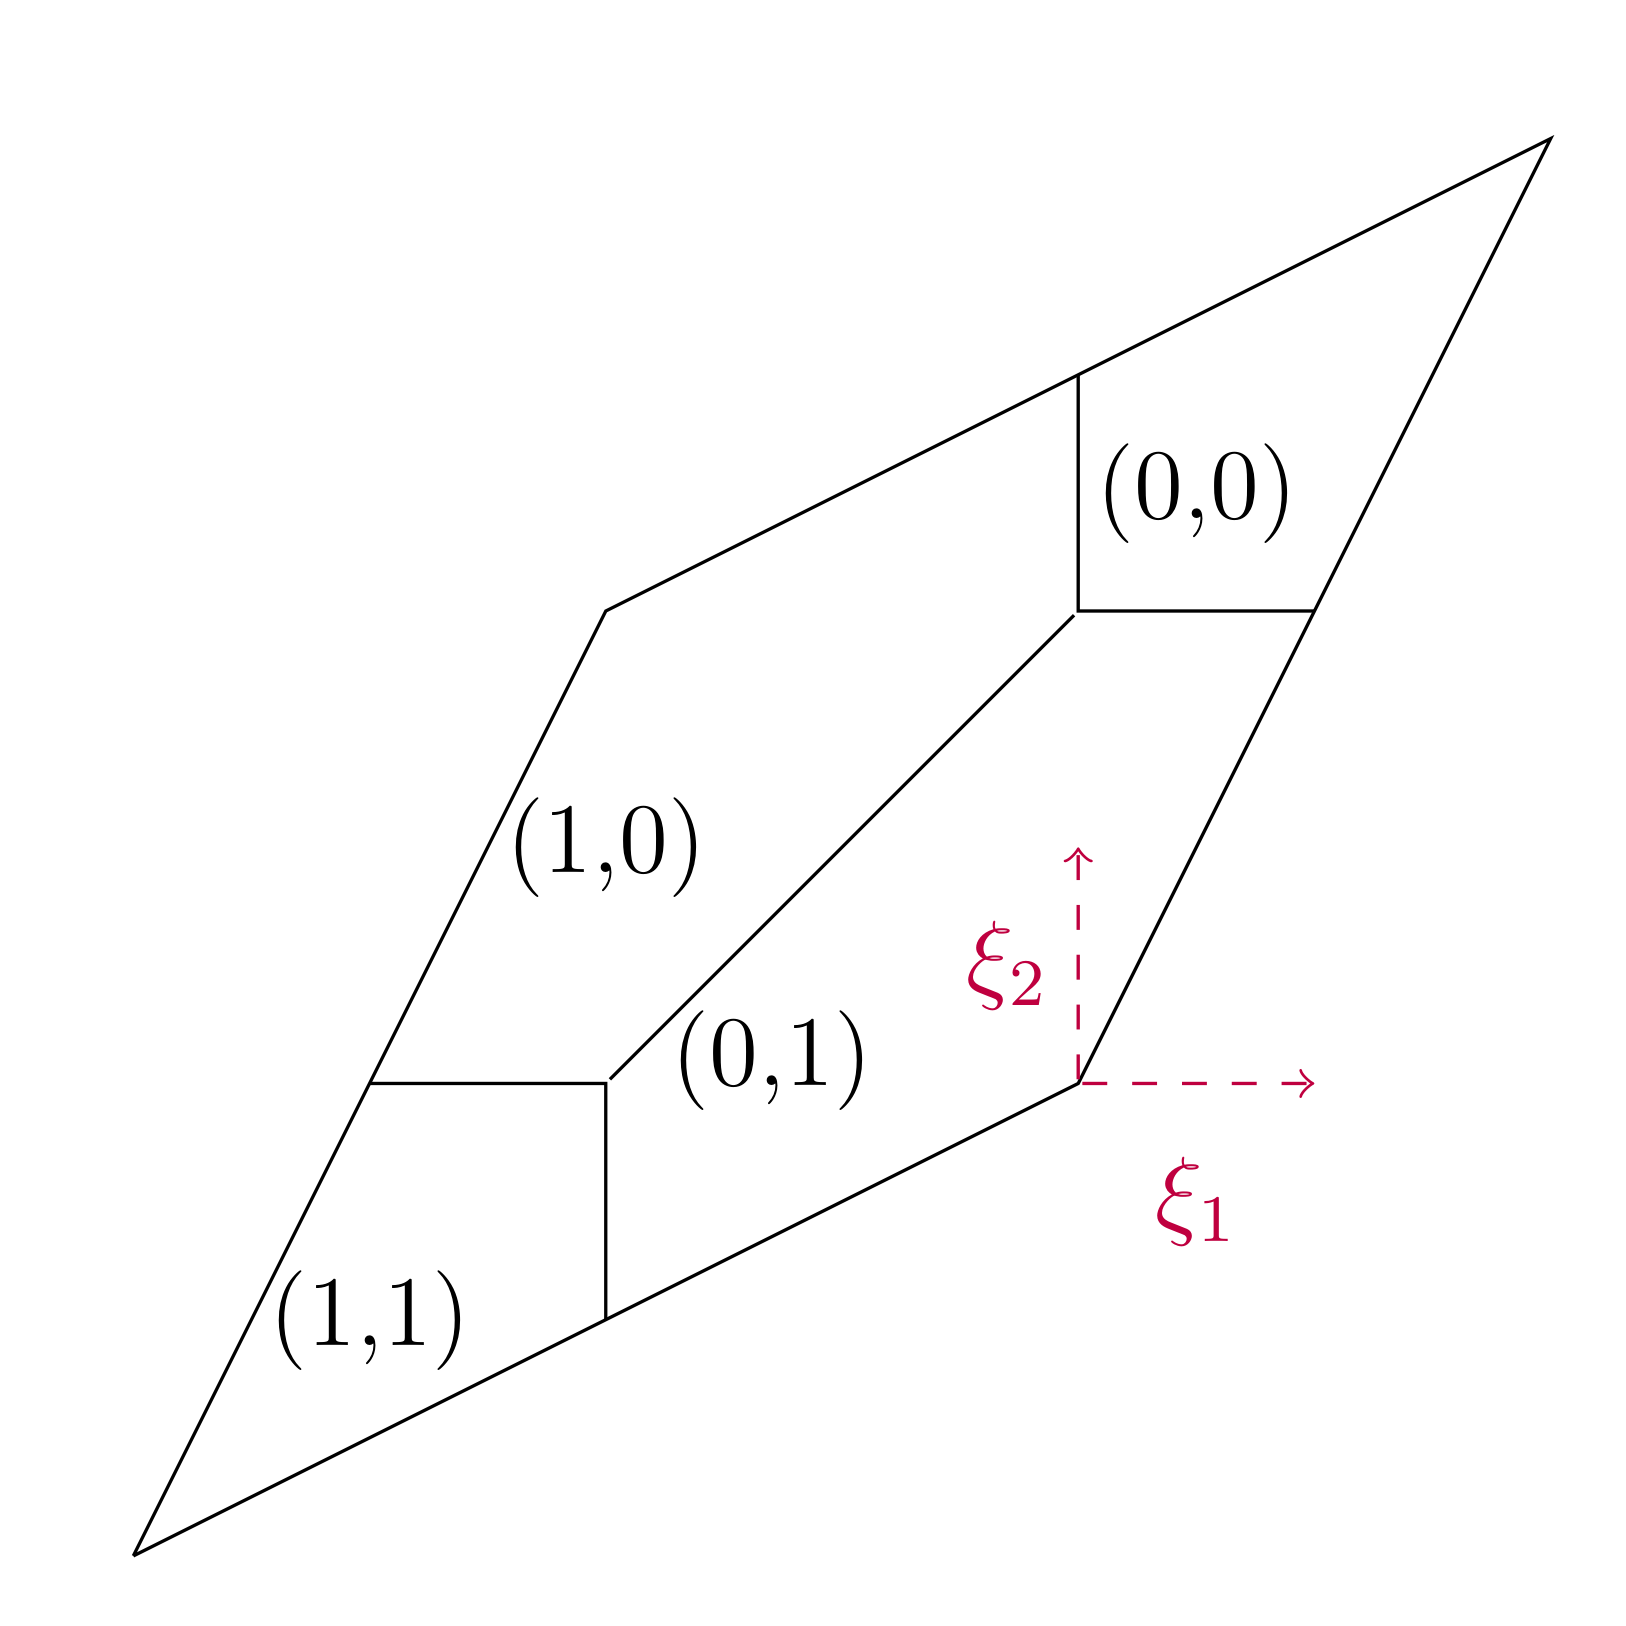
\includegraphics[width=0.40\textwidth]{figures/fig_4_1.png}
\caption{纤维中的单值性，看作平行四边形上的截面
$(\xi_1,\xi_2)\mapsto(\theta_1(\xi_1,\xi_2),\theta_2(\xi_1,\xi_2))$（原书 p.85）}
\label{fig:4-1}
\end{figure}

\begin{remark}[提醒]\label{rem:4-1-15}
下面定义由辛形式导出的作用--角坐标。我们将发现矩映射的像与环簇多面体
（toric polytope）相同，这是 Delzant 定理的一个实例，参见 [MS17]。注意通常的矩映射
落在 $\R^n$ 中（$n$ 为环面的维数），而这里的矩映射落在 $\R^3/\Gamma_B$ 中。
\end{remark}

\begin{claim}[作用--角坐标的定义]\label{clm:4-1-16}
令 $\theta_1:=\arg(x)$、$\theta_2:=\arg(y)$、$\theta_3=\arg(z)$，其中 $x,y,z$ 是复
环簇坐标。它们定义在如下区域中：$|v_0|=|xyz|\le T^\ell$（$\ell$ 充分大），并沿
$v_0\in\R_-$ 去掉一条分支割线；且 $x,y\in(\C^*)^2/\Gamma_B$。于是存在坐标
$\xi_1,\xi_2$ 使
\[
\restr{\omega}{\Vdual}=\de\xi_1\wedge\de\theta_1+\de\xi_2\wedge\de\theta_2,
\]
可简记为 $\de\xi\wedge\de\theta$。注意 $\xi_3,\theta_3$ 不是整体定义的，这正是需要
分支割线的原因。我们还有第三对坐标 $\eta$、$\theta_\eta:=\arg(v_0)$，其中
$\eta=\xi_1+\xi_2+\xi_3$。
\end{claim}

% [Tutor Note: 原书作 |v0|=|xyz| ≤ T^ℓ，其中 T 与 ℓ 的确切含义（阈值与幂次）未
% 说明；结合上下文应理解为 ℓ 充分大时的一个截断区域。保留原样并加译注。]

\begin{proof}
我们有局部 $T^3$-作用。由于 $\theta_i$ 已如上使用，这里改用符号 $\alpha_i$ 作坐标。
\[
\rho\colon T^3\times Y\to Y,\qquad
\rho((\alpha_1,\alpha_2,\alpha_3),(x,y,z))
=(e^{2\pi i\alpha_1}x,e^{2\pi i\alpha_2}y,e^{2\pi i\alpha_3}z).
\]
特别地，在坐标 $v_0$ 上这对应 $e^{2\pi i(\alpha_1+\alpha_2+\alpha_3)}v_0$。当 $v_0$
绕原点转满一圈时，$\theta_1,\theta_2$ 的值已按单值性改变，因此 $v_0$ 上的
$S^1$-作用不是整体定义的。这就是上面要沿割线去掉的原因。

$\alpha_1$ 与 $\alpha_2$ 在 $Y$ 上的无穷小作用由前推 $X_i:=\de\rho(\partial_{\alpha_i})$
（$i=1,2$）表示。若 $\iota_{X_i}\restr{\omega}{\Vdual}$ 是恰当的，比如等于某个函数
$H_i$ 的微分 $\de H_i$（$H_i$ 称为哈密顿量），则称该环面作用是\textbf{哈密顿群作用}
（Hamiltonian group action），而 $(H_1,H_2)$ 就是矩映射。这把我们引向
注~\ref{rem:4-1-15} 中的提醒。在当前设定中，$\omega$
% ===== 原书 p.86 =====
比较复杂，计算 $\iota_{X_i}\restr{\omega}{\Vdual}$ 并不容易。但我们知道：环面
$\R^4/\Lambda$（带 $\Lambda$-周期坐标 $a_1,a_2,a_3,a_4$）上的微分形式由
$\de a_1,\dots,\de a_4$ 在 $\C$ 上生成；由于 $a_i$ 不是整体定义的，这些形式不恰当。
因此存在 $\Gamma_B$-周期函数 $\xi_1,\xi_2$，使
\[
\begin{aligned}
\iota_{X_i}\restr{\omega}{\Vdual}&=\de\xi_i
\ \Longrightarrow\ \restr{\omega}{\Vdual}=\de\xi\wedge\de\theta\\
\Longrightarrow\quad
\iota_{X_i}\Big(\frac{i}{2\pi}\partial\bar\partial F\Big)
&=\frac{i}{2\pi}\de\iota_{X_i}\partial F=\de\xi_i\\
\therefore\quad \xi_1&:=\frac{i}{2\pi}\partial F(2\pi ix\partial_x)
=-\frac{1}{2}xe^{-i\theta_x}\frac{\partial F}{\partial|x|}\\
\therefore\quad \xi_1&=-\frac{1}{4}\frac{\partial F}{\partial|x|^2},
\qquad
\xi_2=-\frac{1}{4}\frac{\partial F}{\partial|y|^2}.
\end{aligned}
\]
其中用到 $\partial\bar\partial=-\bar\partial\partial=-\de\partial$、§2.2 的极坐标
换算，以及 $F$ 作为诸范数的函数在旋转 $x,y,z$ 下不变，故 Lie 导数
$\mathcal{L}_{X_i}\partial F=0$，且 $\partial_{\theta_x}F=0$。要点在于：矩映射
$(\xi_1,\xi_2)$ 给出周期的作用坐标，且由 $F$ 的定义方式，它们关于 $|x|$ 与 $|y|$
单调递增。（但请记住那条提醒：我们把它叫作矩映射，它取值于环面而非仿射空间，这里
是把矩映射的定义扩充到此情形。通常 $\xi_i$ 不应是周期的。）我们看到 $\Vdual$ 辛
同胚于 $(T^4,\omega_{std})$。

注意一条轨道恰为 $(\de\xi_1,\de\xi_2)$ 的核，故矩映射值的原像是一条 $T^2$-轨道。
换一种说法，环面作用保持矩映射。再换一种说法，矩映射纤维的切空间由
$\partial_{\theta_1},\partial_{\theta_2}$ 张成。

注意坐标 $(\xi_1,\xi_2,\eta)$ 以 $\xi\sim\xi+\gamma$ 与 $\eta\ge\varphi(\xi)$ 为周期，
而 $\varphi(\xi+\gamma)=\varphi(\xi)-\kappa(\gamma)+\ip{\xi}{\lambda(\gamma)}$，故当
$\gamma\in\Gamma_B$ 时 $\eta\sim\eta-\kappa(\gamma)+\ip{\xi}{\lambda(\gamma)}$。
\end{proof}

\transnote{$\xi_1,\xi_2$ 是周期的，这是本文「矩映射」一词的非标准之处：它取值于
$\R^3/\Gamma_B$ 而非 $\R^2$。提醒中的「扩充定义」即指此。}

\begin{corollary}\label{cor:4-1-17}
诸 $\ell_k$ 是纤维中的拉格朗日对象。
\end{corollary}

\begin{proof}
$\ell_k$ 是图 $\Gamma_{kM^{-1}(\xi)}$。于是
\[
T\ell_k=\big\langle\partial_{\xi_i}+kM^{-1}(\partial_{\theta_i})\big\rangle_{i=1,2},
\]
且
\[
\omega\big(\partial_{\xi_1}+kM^{-1}(\partial_{\theta_1}),
\partial_{\xi_2}+kM^{-1}(\partial_{\theta_2})\big)=0,
\]
因为 $\omega$ 只从 $\de\xi_1\wedge\de\theta_1$ 或 $\de\xi_2\wedge\de\theta_2$ 取项。
\end{proof}

\transnote{$T\ell_k$ 的两条切向量形如 $\partial_{\xi_i}+kM^{-1}(\partial_{\theta_i})$，
这是「$\ell_k$ 为 $\xi$ 上线性函数的图像」的微分表述：沿 $\xi_i$ 走一步，$\theta$
方向按斜率矩阵 $kM^{-1}$ 同步移动。}

\begin{remark}[记号]\label{rem:4-1-18}
$\mu_X$ 指最后一个坐标上的 $S^1$-作用。$\mu_Y$ 指局部 $T^3$-作用。
\end{remark}

\begin{claim}\label{clm:4-1-19}
（[AAK16]）函数 $\mu_X(x,y)$ 等于由 $(x,y)$ 的轨道所围的盘的面积。
\end{claim}

% ===== 原书 p.87 =====
\begin{proof}
我们断言 $\mu_X(x,y)=\int_D\omega$。这个盘上的积分（例如 $\PP^1$ 的矩映射像是线段，
可在该线段上画出拉长的球面，并把线段中的值映到球面中被扫过部分的面积）是沿如下盘
的积分：其边界分支为一条轨道（$X^{\#}$ 的积分流）以及从 $(x,y)$ 绕回原点的直线。
称该直线为 $C$。于是可把积分写成
\[
\int_C\iota_{X^{\#}}\omega=\int_C\de\mu_X=\mu_X(x,y)-\mu_X(0,0)=\mu_X(x,y).
\]
\end{proof}

\transnote{此处「盘的面积」按 $\PP^1$ 的矩映射像为线段来理解：线段上每个值对应球面
被扫过部分的面积，于是边界积分化为矩映射值之差。}

\begin{remark}\label{rem:4-1-20}
我们的出发点多面体，并希望它成为某个待构造辛形式下的矩映射像。特别地，我们要找
一个辛形式，使六边形的边界 $\PP^1$ 长度为 $1$。
\end{remark}

\medskip\noindent\textbf{单值性计算}\par
\begin{example}[降一维：二维局部情形]\label{ex:4-1-21}
$\C^2$ 带辛纤维丛 $(x,y)\mapsto xy$ 的情形即 Lefschetz 纤维丛的设定：奇异纤维由
$x=0$ 与 $y=0$ 给出的两份 $\C$ 构成，单值性是绕圆柱形纤维腰部 $S^1$ 的 Dehn 扭转。
Reference.
\end{example}

% [Tutor Note: 原书此处仅有「Reference.」一词，未给出具体文献，保留原样。]

\transnote{二维局部情形是 Lefschetz 纤维丛的标准图像：纤维是圆柱，奇异纤维为两份
$\C$ 沿原点粘合，单值性为绕腰部 $S^1$ 的 Dehn 扭转。下一例把这一图像逐坐标实现。}

$f(x,y)=xy$，$S^1$-作用为 $(e^{i\theta}x,e^{-i\theta}y)$。对应的全纯向量场是
$iz_1\partial_{z_1}-iz_2\partial_{z_2}$，它与
$\omega=\frac{i}{2}(\de z_1\wedge\de\bar z_1+\de z_2\wedge\de\bar z_2)$ 缩并给出
哈密顿向量场 $-\frac{1}{2}(|z_1|^2-|z_2|^2)$。我们在二维纤维上有一组新坐标：矩映射
坐标 $\mu$ 与作用的角坐标 $\theta$。当 $xy\to0$ 时，$\mu$-高度为 $0$ 的轨道，即
$|x|=|y|$ 处，趋于零。由此可以看出，为什么我们得到的是颈部收缩为零的圆柱图像。

\begin{example}[三维局部情形]\label{ex:4-1-22}
分几步来做。

\begin{itemize}[leftmargin=2.2em,itemsep=0.25em]
\item \textbf{全纯纤维丛的平行移动。} 设
\begin{equation}\label{eq:4-1}
\begin{aligned}
f&=xyz, & |f|^2&=(x_1^2+x_2^2)(y_1^2+y_2^2)(z_1^2+z_2^2)\\
\nabla_{\omega_0}f&=2\langle x|yz|^2,\;y|xz|^2,\;z|xy|^2\rangle\\
&\ \perp\ (|f|^2)^{-1}(c^2)=\{|xyz|=c\}
\end{aligned}
\end{equation}
于是 $|f|^2$ 的梯度向量场的投影与此情形中的圆垂直。特别地，乘以 $i$ 就得到与圆相切
的东西。乘以 $i$ 恰好给出正确的水平提升，这一点成立是因为 $f$ 全纯，从而与 $i$
交换。此外我们还会看到，梯度是水平子空间中元素的线性组合。

\transnote{这一步的三个算式各有分工：先求 $|f|^2$ 的梯度，它垂直于水平圆；乘 $i$
得切向；最后除以标量 $g$，使 $\de f(X_H)=iw\partial/\partial w$，从而 $X_H$ 覆盖
底空间中的圆。}

\item \textbf{求水平子空间。}
\begin{claim}\label{clm:4-1-23}
$X_{\Re(f)},X_{\Im(f)}\in H$，其中 $H$ 是水平分布。
\end{claim}

\begin{proof}
纤维恰为 $f$ 的水平集。
\begin{equation}\label{eq:4-2}
\begin{aligned}
\ker(d_pf)&=T_p(f^{-1}(c)),\qquad p\in f^{-1}(c)\\
\ker(\de f)&=\ker(\de\Re(f))\cap\ker(\de\Im(f))\\
\ker(\de\Re(f)(\cdot))&=\ker(\omega_0(X_{\Re(f)},\cdot))\ni X_{\Re(f)}\\
f\ \text{全纯}\ \Longrightarrow\ \nabla(\Re(f))&=-J\nabla(\Im(f))\\
\therefore\ \nabla(\Re(f))&=-JX_{\Re(f)}=X_{\Im(f)}
\ \Longrightarrow\ X_{\Im(f)}\in\ker(\de\Re(f))\\
\therefore\ H&=\big\langle X_{\Re(f)},X_{\Im(f)}\big\rangle
=\big\langle\nabla(\Re(f)),\nabla(\Im(f))\big\rangle
\end{aligned}
\end{equation}
\end{proof}

\item \textbf{平行移动的计算。} 把 $i$ 乘梯度作适当缩放后积分其水平提升，因为我们要
覆盖底空间中的圆。
\begin{equation}\label{eq:4-3}
\begin{aligned}
i\nabla(|f|^2)&=2i\langle\nabla\Re(f),\nabla\Im(f)\rangle\in Hor\\
&=2i\big\langle x_1|y|^2|z|^2,\;x_2|y|^2|z|^2,\;y_1|x|^2|z|^2,\;
y_2|x|^2|z|^2,\;z_1|x|^2|y|^2,\;z_2|x|^2|y|^2\big\rangle\\
\int_0^\theta i\nabla(|f|^2)&=\rho^{i\nabla(|f|^2)}(\theta)
=\big(e^{2i\theta|y|^2|z|^2}x,\;e^{2i\theta|x|^2|z|^2}y,\;
e^{2i\theta|x|^2|y|^2}z\big)
\end{aligned}
\end{equation}
\end{itemize}
\end{example}

% ===== 原书 p.88 =====
我们要找 $\frac{\partial}{\partial\theta}e^{i\theta}=iw\partial/\partial w$ 的水平提升。
即找一个适当的标量函数 $g$，使 $\de f(i(\nabla|f|^2)/g)=iw\partial/\partial w$。
\begin{align*}
\de f&=yz\,\de x+xz\,\de y+xy\,\de z\\
\nabla_{g_0}|f|^2&=2\langle x|yz|^2,\;y|xz|^2,\;z|xy|^2\rangle\\
|\nabla|f|^2|^2&=4|xyz|^2\big(|yz|^2+|xz|^2+|xy|^2\big)\\
\Longrightarrow\quad
\big(|yz|^2+|xz|^2+|xy|^2\big)&=\frac{|\nabla|f|^2|^2}{4|f|^2}\\
X_H&=\frac{2i}{g}\langle x|yz|^2,\;y|xz|^2,\;z|xy|^2\rangle
\quad\text{s.t.}\quad \de f(X_H)=iw\partial/\partial w\\
\therefore\quad
\frac{2i}{g}xyz\big(|yz|^2+|xz|^2+|xy|^2\big)&=iw=i(xyz)
\ \Longrightarrow\ g=2\big(|yz|^2+|xz|^2+|xy|^2\big)\\
\therefore\quad X_H&=\frac{i}{|yz|^2+|xz|^2+|xy|^2}
\langle x|yz|^2,\;y|xz|^2,\;z|xy|^2\rangle.
\end{align*}
于是
\begin{equation}\label{eq:4-4}
\begin{aligned}[b]
\therefore\quad \rho^{X_H}(x,y,z,\theta)
&=\Big(e^{i\theta\frac{|y|^2|z|^2}{|y|^2|z|^2+|x|^2|z|^2+|x|^2|y|^2}}x,\;
 e^{i\theta\frac{|x|^2|z|^2}{|y|^2|z|^2+|x|^2|z|^2+|x|^2|y|^2}}y,\\
&\qquad\qquad\qquad
 e^{i\theta\frac{|x|^2|y|^2}{|y|^2|z|^2+|x|^2|z|^2+|x|^2|y|^2}}z\Big)\\
&=\Big(e^{i\theta\frac{|x|^{-2}}{|x|^{-2}+|y|^{-2}+|z|^{-2}}}x,\;
 e^{i\theta\frac{|y|^{-2}}{|x|^{-2}+|y|^{-2}+|z|^{-2}}}y,\\
&\qquad\qquad\qquad
 e^{i\theta\frac{|z|^{-2}}{|x|^{-2}+|y|^{-2}+|z|^{-2}}}z\Big).
\end{aligned}
\end{equation}

% ===== 原书 p.89 =====
这里用到圆上 $w=xyz$，最后一步则除以 $|f|^2$，以便更容易看出 Dehn 扭转的行为。
这就给出本节开头的单值性结果，即引理~\ref{lem:4-1-11}。

\begin{example}[本文 $v_0\colon Y\to\C$ 的设定]\label{ex:4-1-24}
\end{example}

\begin{claim}\label{clm:4-1-25}
若 $\gamma(t)(v_0)=e^{2\pi it}v_0$，则 $\gamma'$ 的水平提升形如
\[
X_{hor}=\partial/\partial\theta_{v_0}+f(\xi)\partial/\partial\theta_1
+g(\xi)\partial/\partial\theta_2.
\]
\end{claim}

\begin{proof}
注意 $\operatorname{Lie}T^3$ 上的 Lie 括号为零，故标准理论给出
\[
\omega(X_{\zeta_1},X_{\zeta_2})=X_{[\zeta_1,\zeta_2]}=0.
\]
特别地，若取 $\zeta_1=(1,0,0)$ 或 $(0,1,0)$，即 $TF$ 的角切向（$F$ 为 $v_0$ 的
纤维），而 $\zeta_2$ 任意，则得零。又因 $\omega(X_{(1,0,0)},-)=\de\xi_1$，可见
$X_{\zeta_2}$ 不含 $\partial/\partial\xi_1$ 分量；换言之，它的流保持矩映射坐标
$\xi_1$ 与 $\xi_2$。

特别地，设 $X_{hor}$ 为断言中的水平提升。设 $X_{(1,0,0)}$ 为旋转 $x$ 坐标（保持
$y$ 与 $v_0$ 不动）的无穷小作用生成的向量场。于是 $X_{hor}$ 的水平性（按矩映射
$\xi_1$ 的定义）给出
\[
\de\xi_1(X_{hor})=\omega(X_{(1,0,0)},X_{hor})=0.
\]
因此若 $\phi_t$ 是 $X_{hor}$ 的流，由链式法则得
\[
\frac{\de}{\de t}(\xi_1\circ\phi_t)=0
\qquad\therefore\quad \xi_1\circ\phi_t=\xi_1,
\]
对 $\xi_2$ 同理。故平行移动保持矩映射坐标 $\xi_1,\xi_2$。它还保持 $\eta$，因为我们
考虑的是角向平行移动。于是在坐标
$\pi\colon(\xi_1,\xi_2,\eta,\theta_x,\theta_y,\theta_{v_0})\to(|w|,\theta_w)
:=(|v_0|,\theta_{v_0})$ 下（$w$ 为 $v_0\colon Y\to\C$ 底空间 $\C$ 上的坐标），
\[
\de\pi(X_{hor})=\partial/\partial\theta_{v_0}
\]
\[
\Longrightarrow\quad
\begin{pmatrix}
0&0&\partial|v_0|/\partial\eta&0&0&0\\
0&0&0&0&0&1
\end{pmatrix}
\begin{pmatrix}0\\0\\h\\f\\g\\a\end{pmatrix}
=\begin{pmatrix}h\,\partial|v_0|/\partial\eta\\ a\end{pmatrix}=(0,1),
\]
故 $a=1$、$h=0$，因为 $\eta$ 依赖于 $|v_0|$。于是水平提升取如下形式：
\[
X_{hor}=\partial/\partial\theta_{v_0}+f\partial/\partial\theta_1
+g\partial/\partial\theta_2.
\]
\end{proof}

% ===== 原书 p.90 =====
\begin{corollary}\label{cor:4-1-26}
$X_{hor}=\partial/\partial\theta_{v_0}+f\partial/\partial\theta_1
+g\partial/\partial\theta_2$，其中 $f$ 与 $g$ 只是 $\xi_1,\xi_2$ 的函数。
\end{corollary}

\begin{proof}
注意：由矩映射在径向平行移动下的不变性，可得与 $\eta$ 无关。设 $\rho^t$ 为来自
角向平行移动的水平向量场 $X_{hor}$ 的流：
\[
\rho^t(\xi_1,\xi_2,\eta,\theta_1,\theta_2,\theta_{v_0})
=(\xi_1,\xi_2,\eta,\theta_1+tf,\theta_2+tg,\theta_{v_0}+t).
\]
设 $\phi_\alpha$ 为 $T^2$-作用 $(e^{2\pi i\alpha_1}x,e^{2\pi i\alpha_2}y,v_0)$。它是
辛同胚：因为全纯且保持诸范数，故与 $\partial\bar\partial$ 交换并保持凯勒势 $F$，从而
$(\phi_\alpha)_*\partial\bar\partial F=\partial\bar\partial F$。它还是逐纤维的辛同胚，
因为它在纤维上作用。于是
\begin{align*}
0&=\phi_\alpha^*\omega(TF,H)=\omega((\phi_\alpha)_*TF,(\phi_\alpha)_*H)\\
&=\omega(TF,(\phi_\alpha)_*H)\\
&\qquad\therefore\quad (\phi_\alpha)_*H=H\\
\de\pi((\phi_\alpha)_*X_{hor})&=\de(\pi\circ\phi_\alpha)(X_{hor})=\de\pi(X_{hor})\\
&\qquad\therefore\quad (\phi_\alpha)_*(X_{hor})\circ\phi_\alpha^{-1}=X_{hor}\\
\Longrightarrow\quad \de\phi_\alpha\Big(\frac{\de}{\de t}\rho^t\Big)\circ\phi_\alpha^{-1}
&=\frac{\de}{\de t}(\phi_\alpha\circ\rho^t)\circ\phi_\alpha^{-1}\\
&=\frac{\de}{\de t}(\rho^t)\\
\Longrightarrow\quad \phi_\alpha\circ\rho^t&=\rho^t\circ\phi_\alpha\\
\Longrightarrow\quad
&(\xi_1,\xi_2,\eta,\theta_1+\alpha_1+tf(\xi,\theta+\alpha),\\
&\qquad \theta_2+\alpha_2+tg(\xi,\theta+\alpha),\theta_{v_0}+t)\\
&=
(\xi_1,\xi_2,\eta,\theta_1+\alpha_1+tf(\xi,\theta),\\
&\qquad \theta_2+\alpha_2+tg(\xi,\theta),\theta_{v_0}+t)\\
\Longrightarrow\quad f(\xi,\theta+\alpha)=f(\xi,\theta),\quad
g(\xi,\theta+\alpha)&=g(\xi,\theta)\quad\forall\alpha
\end{align*}
其中我们沿 $\frac{\de}{\de t}$ 积分得到下一行。于是 $f$ 与 $g$ 与 $\theta_1,\theta_2$
无关。类似的论证表明它们也与 $\theta_{v_0}$ 无关，即对 $v_0$ 坐标上的 $S^1$-作用
$\phi_\lambda$（$\lambda\in S^1$）有 $\phi_\lambda\circ\rho^t=\rho^t\circ\phi_\lambda$。
\end{proof}

\medskip\noindent\textbf{与线性拉格朗日哈密顿同痕的纤维拉格朗日}\par
\begin{definition}\label{def:4-1-27}
令 $L_i$ 为纤维中 $\ell_i$ 沿 U 形曲线的平行移动。
\end{definition}

\begin{claim}\label{clm:4-1-28}
平行移动后的 $\ell_i$ 与 $\ell_{i+1}$ 哈密顿同痕。
\end{claim}

\begin{proof}
我们在纤维中构造同痕 $\psi_t\colon F\to F$（坐标 $(\xi_1,\xi_2,\theta_1,\theta_2)$）。
它把 $\ell_1$ 映到 $\phi(\ell_0)$，其中 $\phi$ 是单值性。为证 $\psi_t$ 是哈密顿
同痕，即 $\iota_{\frac{\de}{\de t}\psi_t}\omega=\de H_t$ 对某 $H_t$ 成立，Banyaga
的结果（参见 Pascaleff 讲义）表明只须证明：$\omega$ 经由 $H_1(F)$ 的生成元扫出的
圆柱的通量为零。
\[
\Big\langle\int_t\iota_{X_t}\omega,[\gamma]\Big\rangle
=\ip{\operatorname{Flux}(\psi_t)}{[\gamma]}
=\int_{\psi_t(\gamma)}\omega
=\text{$\gamma$ 随时间扫出的圆柱的面积}.
\]
% ===== 原书 p.91 上部（§4.1 收尾；§4.2 起属下块） =====
先定义同痕，并令 $A:=M^{-1}$。
\[
\psi_t(\xi_1,\xi_2,\theta_1,\theta_2)
:=(\xi_1,\xi_2,\theta_1+t(f(\xi)-A_1\xi),\theta_2+t(g(\xi)-A_2\xi)).
\]

\transnote{减去 $A\xi$ 是为了去掉线性拉格朗日 $\ell_1$ 自身的斜率：$A=M^{-1}$ 正是
该斜率矩阵，故 $\psi_t$ 从恒等出发，在 $t=1$ 时把线性图拉成平行移动后的图。}
注意 $H_1(F)$ 的秩为四，因为 $F\iso T_B\times T_F$。若取 $\gamma$ 为
$(0,0,1,0)$ 或 $(0,0,0,1)$ 生成的两个角向中的回路，则 $\{\psi_t(\gamma)\}_t$ 是一维
的，因为 $\xi$ 为常数，故积分为零。今取
\[
\gamma(t)=(2t,t,0,0),\qquad -\frac{1}{2}\le t\le\frac{1}{2}.
\]
$\gamma(t)=(t,2t,0,0)$ 的情形类似。
\begin{align*}
\operatorname{flux}&=\int_{\psi_t(\gamma)}\omega=\int_\gamma\iota_{X_t}\omega
=\int_\gamma(\de\xi_1\wedge\de\theta_1+\de\xi_2\wedge\de\theta_2)
\big((f-A_1)\partial_{\theta_1}+(g-A_2)\partial_{\theta_2},-\big)\\
&=\int_\gamma(f-A_1)\de\xi_1+(g-A_2)\de\xi_2
=\int_{-1/2}^{1/2}2f(2t,t)\,\de t+g(2t,t)\,\de t,
\end{align*}
其中用到 $A$ 是线性映射这一事实所蕴含的关于零点的对称性；剩下要证上式为零，即
$f$ 与 $g$ 关于零点的对称性。只须证明 $f(-\xi)=-f(\xi)$，对 $g$ 同理。

为此回忆 $f$ 与 $g$ 由
\[
X_{hor}=\frac{\partial}{\partial\theta_{v_0}}
+f(\xi)\frac{\partial}{\partial\theta_1}
+g(\xi)\frac{\partial}{\partial\theta_2}
\]
定义。也回忆 $X_{hor}$ 被任何保纤维的辛同胚保持，正如上面 $T^2$-作用的例子所示。
另一个保纤维的辛同胚是纤维中的
$\phi_{neg}\colon(\xi,\theta)\mapsto(-\xi,-\theta)$。它是辛同胚，因为
$\de\xi\wedge\de\theta\mapsto\de(-\xi)\wedge\de(-\theta)=\de\xi\wedge\de\theta$。
于是
\[
(\phi_{neg})_*(X_{hor})=X_{hor}\circ\phi_{neg}
\qquad\Longrightarrow\quad f(-\xi)=-f(\xi),\quad g(-\xi)=-g(\xi).
\]
这就完成了证明。
\end{proof}

\transnote{「通量为零」是同痕可写成哈密顿流的判据（Banyaga 定理），本文只须对
$H_1(F)$ 的生成元验证。末尾的 $\phi_{neg}$ 论证把 $f,g$ 的对称性化归为 $X_{hor}$
在保纤维辛同胚下的不变性。}
